\documentclass[11pt, a4paper]{article}
\usepackage{graphicx}
\usepackage{amsmath}
\usepackage{listings}
\usepackage{url}

\title{Assignment 4: Fourier Approximations} % Title

\author{Munir Ahamed M [EE20B086]} % Author name

\date{26th February2022} % Date for the report
\begin{document}	
		
\maketitle % Insert the title, author and date
\section*{Abstract}
%Create new section;it is autonumbered
The aim of this assignment is :
\begin{itemize}
\item To find the Fourier series of the functions $e^{x}$ and $cos(cos(x))$ using integration and least squares method.
\item To estimate the error in case of least squares approximation and to find it's deviation for given functions.
\item To plot graphs to understand the above.
\end{itemize}


\section{Plotting $e^{x}$ and $cos(cos(x))$}
The following python snippet is used to declare the functions $e^{x}$ and $cos(cos(x))$, also a (the independent variable) values are declared from -2$\pi$ to 4$\pi$.

\begin{verbatim}
def exponent(x):                     #defining function to calculate exp(x)
    return exp(x)

def cosofcos(x):                     #defining function to calculate cos(cosx)
    return (cos(cos(x)))
	
a = linspace(-2*pi,4*pi,600)         #calculating function values and different
a_p = tile(linspace(0,2*pi,200), 3)  #intervals between -2pi to 4pi.
y1 = exponent(a)                                                                                                     
y1_p = exponent(a_p)                 #as exp(x) is not periodic, y1_p denotes
y2 = cosofcos(a)                     #it's periodic extension.
\end{verbatim}
The following code plots $e^{x}$, it's periodic extension and $cos(cos(x))$.
\begin{verbatim}
figure(1)                            #plotting exp(x) function's true value
semilogy(a,y1, label='True value')
semilogy(a,y1_p, label='Periodic extension')
title("exp(x) semilog", size=18)
xlabel(r'$x\rightarrow$', size=18)
ylabel(r'$e^x\rightarrow$', size=18)
grid(True)
legend()

figure(2)                            #plotting cos(cosx) function's true value
plot(a,y2, label='True value')
title("cos(cos(x))", size=18)
xlabel(r'$x\rightarrow$', size=18)
ylabel(r'$cos(cos(x))\rightarrow$', size=18)
grid(True)
legend()
\end{verbatim}
The plots of $e^{x}$ and $cos(cos(x))$ are shown below, as $e^{x}$ is not periodic it has a periodic extension and it is shown in the corresponding figure :
   \begin{figure}[!tbh]
   	\centering
   	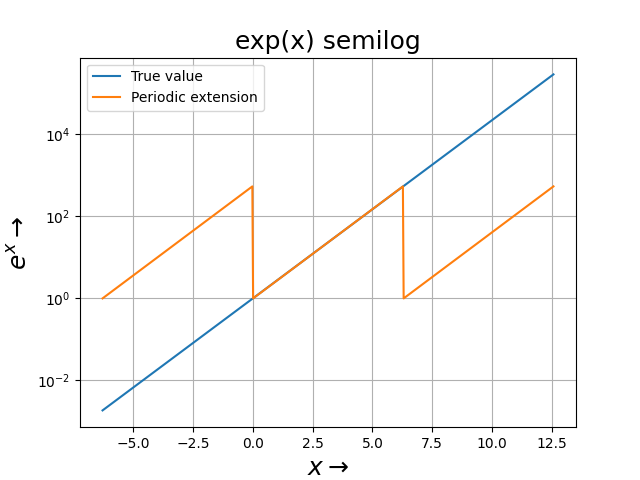
\includegraphics[scale=0.6]{Figure_1a.png}   
   	\caption{Data plot}
   	\label{fig:sample}
   \end{figure} 
   
   \begin{figure}[!tbh]
   	\centering
   	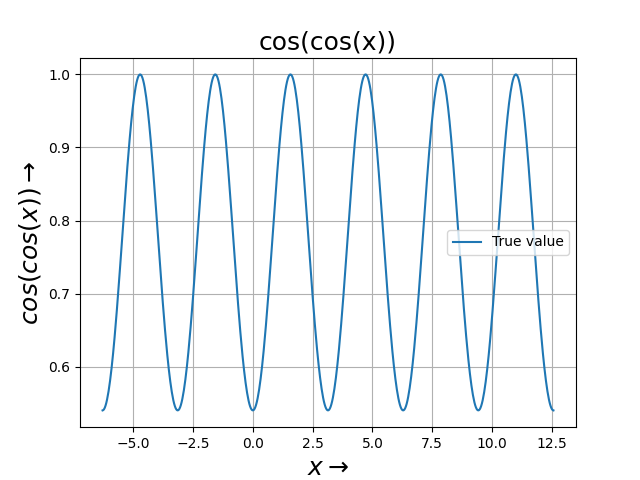
\includegraphics[scale=0.6]{Figure_2a.png}   
   	\caption{Data plot}
   	\label{fig:sample}
   \end{figure}
   
The calculation of f(x) based on least squares is discussed in the final part of the report.
\newpage
\section{The Fourier coefficients}
The fourier series of a function is given by:
\begin{equation}
    a_{0} + \sum\limits_{n=1}^{\infty} {{a_{n}\cos(nx_{i})+b_{n}\sin(nx_{i})}} \approx f(x_{i}) 
    \end{equation}
    	To find the Fourier coefficients we use:
    \begin{equation}
         a_{0} = \frac{1}{2\pi}\int\limits_{0}^{2\pi} f(x)dx 
    \end{equation}
    \begin{equation}
         a_{n} = \frac{1}{\pi}\int\limits_{0}^{2\pi} f(x)\cos(nx)dx 
    \end{equation}
    \begin{equation}
         b_{n} = \frac{1}{\pi}\int\limits_{0}^{2\pi} f(x)\sin(nx)dx 
    \end{equation}

In python the above coefficients are calculated using \textit{quad()} function to perform an intergration . We declare the functions below which will be used to calculate the intergral while determining the fourier coefficients :
\begin{verbatim}
def u_exponent(x,k):                  #defining function to calculate 
    return (exp(x)*cos(k*x))          #f(x)*cos(kx) and f(x)*sin(kx)

def v_exponent(x,k):
    return (exp(x)*sin(k*x))

def u_cosofcos(x,k):
    return (cos(cos(x))*cos(k*x))

def v_cosofcos(x,k):
    return (cos(cos(x))*sin(k*x))
\end{verbatim}
The python code snippet for finding the fourier coefficients is:
\begin{verbatim}
a_0 = integrate.quad(exponent, 0, 2*pi)[0]/(2*pi)
fn1 = [a_0]
a_0 = integrate.quad(cosofcos, 0, 2*pi)[0]/(2*pi)
fn2 = [a_0]

for k in range(1,26):   #loading fn1, fn2 with coeff. of corresponding func.
    u = integrate.quad(u_exponent, 0, 2*pi, args=(k))[0]/pi
    v = integrate.quad(v_exponent, 0, 2*pi, args=(k))[0]/pi
    fn1.extend([u,v])
    u = integrate.quad(u_cosofcos, 0, 2*pi, args=(k))[0]/pi
    v = integrate.quad(v_cosofcos, 0, 2*pi, args=(k))[0]/pi
    fn2.extend([u,v])
\end{verbatim}
Here variable k is passed as the argument for integration.
  
\section{Fourier coefficients Plots}
Plots for the Fourier coefficients of $e^{x}$ and $cos(cos(x))$ :
	\begin{figure}[!tbh]
   	\centering
   	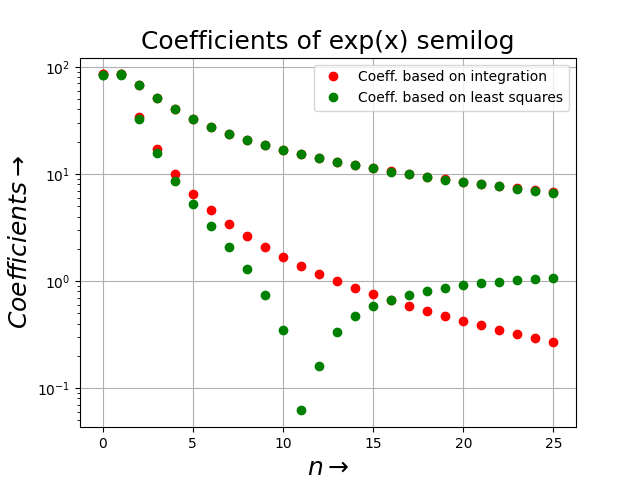
\includegraphics[scale=0.6]{Figure_3.png}   
   	\caption{Semilog plot of the fourier coefficients of $e^{x}$}
   	\label{fig:sample}
   \end{figure} 

	\begin{figure}[!tbh]
   	\centering
   	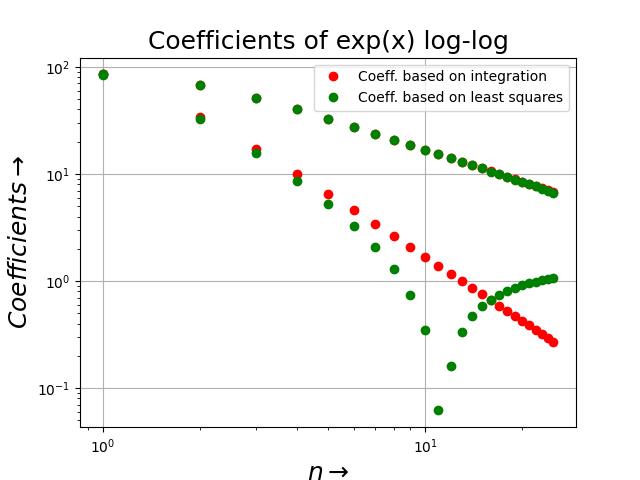
\includegraphics[scale=0.6]{Figure_4.png}   
   	\caption{Log plot of the fourier coefficients of $e^{x}$}
   	\label{fig:sample}
   \end{figure} 
 
	\begin{figure}[!tbh]
   	\centering
   	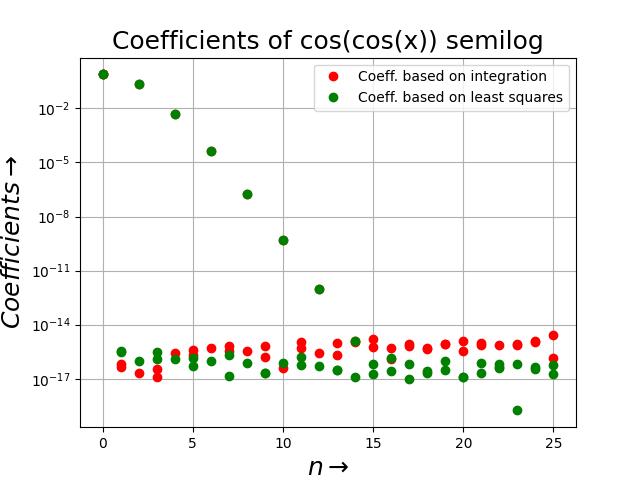
\includegraphics[scale=0.6]{Figure_5.png}   
   	\caption{Semilog plot of the fourier coefficients of $cos(cos(x))$}
   	\label{fig:sample}
   \end{figure} 

	\begin{figure}[!tbh]
   	\centering
   	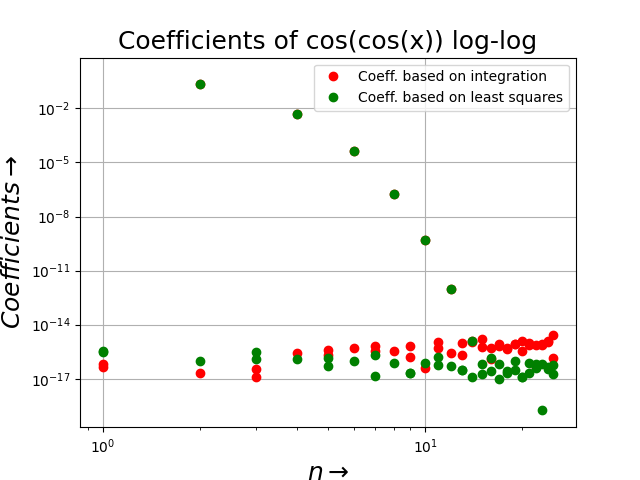
\includegraphics[scale=0.6]{Figure_6.png}   
   	\caption{Log plot of the fourier coefficients of $cos(cos(x))$}
   	\label{fig:sample}
   \end{figure} 

a. From the plots (based on integration) we observe that $b_n$ is nearly zero for $cos(cos(x))$. As $cos(cos(x))$ is an even function all the $b_n$ terms should be zero for the Fourier expansion to be an even function as well.\\\\
b. The magnitude of the coefficients would represent how much of certain frequencies happen to be in the output. $cos(cos(x))$ does not have very many frequencies of harmonics, so it dies out quickly. However, since the periodic extension of $e^{x}$ is discontinuous. To represent this discontinuity as a sum of continuous sinusoids, we would need high frequency components, hence coefficients do not decay as quickly.\\\\
c. The loglog plot is linear for $e^{x}$ since Fourier coefficients of $e^{x}$ decay with $1/n$ or $1/n^{2}$. The semilog plot seems linear in the $cos(cos(x))$ case as its fourier coefficients decay exponentially with n.

\section{The Least Squares Approach}
In the least squares approach, we'll create matrices A and b, and then use \textit{lstsq()} function to get the most approximate values of the fourier coefficients.\\
The python code snippet to create the matrices and to get the least squared value of the coefficients :
\begin{verbatim}	
A = empty((400,51))             #creating empty A matrix to solve for c
x = linspace(0, 2*pi, 401)
x = x[:-1]

for i in range(400):
    A[i][0] = 1
    for k in range(1,26):
        A[i][2*k-1] = cos(k*x[i])
        A[i][2*k] = sin(k*x[i])

b1 = empty((400,1))
b2 = empty((400,1))

for k in range(400):            #b matrix which contains function values
    b1[k][0] = exponent(x[k])
    b2[k][0] = cosofcos(x[k])

c1 = lstsq(A,b1,rcond=None)[0]  #obtaining coeff. by least squares
c2 = lstsq(A,b2,rcond=None)[0]
\end{verbatim}
The green circled plot in figures 2-6 denote the coefficients obtained by least squares. 
     
\section{Deviation from Actual Values} 
The least squares approach is still an approximate method and will definitely have a slight deviation from the actual value.\\
The following python code snippet is used to calculate the deviation:
\begin{verbatim}	
dev_exp = transpose(abs(fn1-transpose(c1))) #finding deviations of coeff.
devmax_exp = max(dev_exp)                   #by both methods and finding max
dev_coc = transpose(abs(fn2-transpose(c2)))
devmax_coc = max(dev_coc)
\end{verbatim}
The deviation in the case of $e^{x}$ is 1.332731\\
The deviation in the case of $cos(cos(x))$ is 0.000000\\\\
There is very good agreement in values in the case of $cos(cos(x))$ but a significant amount of difference in the case of $e^{t}$. The reason for this is that the periodic extension of the exponential function is discontinuous, and hence would require a lot more samples to accurately determine its Fourier coefficients. If we increased the number of samples to $10^{6}$, the maximum deviation would reduce, but not vanish.
The effect of this lack of samples is felt more near the discontinuity of the signal.


\section{Estimated Functions}
Using the predicted values of the fourier coefficients, we can calculate the functional values for both $e^{x}$ and $cos(cos(x))$. \\
The plots showing both the actual and predicted functional values are as shown below:

 	\begin{figure}[!tbh]
   	\centering
   	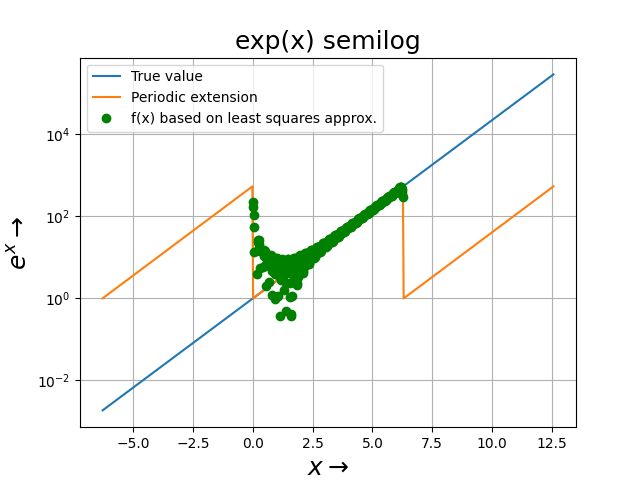
\includegraphics[scale=0.6]{Figure_1.png}   
   	\caption{Actual and predicted values for $e^{x}$}
   	\label{fig:sample}
   \end{figure} 
   
   \begin{figure}[!tbh]
   	\centering
   	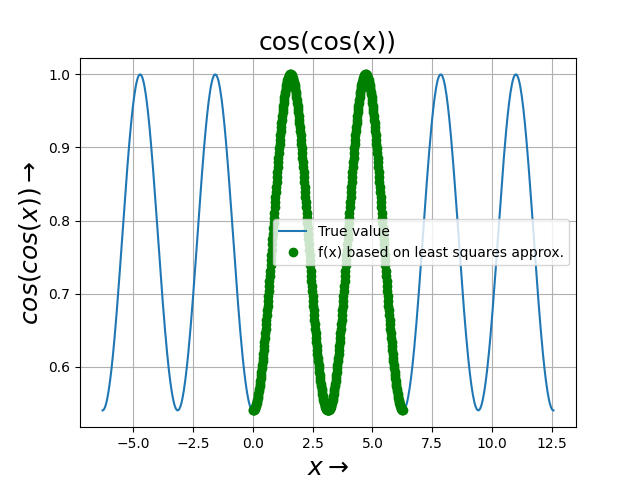
\includegraphics[scale=0.6]{Figure_2.png}   
   	\caption{Actual and predicted values for $cos(cos(x))$}
   	\label{fig:sample}
   \end{figure} 
   The $cos(cos(t))$ vs t graph, agrees almost perfectly, beyond the scope of the precision of the least squares fitter.
The Fourier approximation of $e^{t}$ does not agree very well to the ideal case near the discontinuity. The cause for this is the Gibbs Phenomenon, which can be described as below.
The partial sums of the Fourier series will have large oscillations near the discontinuity of the function. These oscillations do not die out as n increases, but approaches a finite limit.
This is one of the causes of ringing artifacts in signal processing, and is very undesirable.
Plotting the output on a linear graph would make this ringing much more apparent.
	
\section*{Conclusions}
\begin{itemize}
\item We saw two different ways to calculate the Fourier series of a periodic signal.
\item We saw how least squares fitting can be used to simplify the process of calculating the Fourier Series.
\item We observed Gibbs phenomenon at the discontinuity in the Fourier approximation of $e^{t}$.
\end{itemize}

\end{document}